\section{Results}

\subsection{Study population and matching}

Of 452,863 admissions in the cleaned data, 384,334 had an ischaemic stroke with a recorded discharge mRS and did not receive IVT after MT, and 343,739 of these had an arrival NIHSS of 1 to 25 (Supplementary Figure~\ref{fig:supp_flow}). Of the 343,739, 58,074 received IVT and/or MT and 285,665 received neither. Five of the 39 trial groups (IVT late (perfusion)) had no treated patients. In the remaining 34 groups, 54,637 of 54,703 treated patients (99.9\%) were matched to an untreated control, and group sizes ranged from 51 to 13,618 matched pairs (Supplementary Table~\ref{tab:supp_matching}). A further 3,371 treated patients did not fit any trial group (for example, MT in NIHSS 1--10). Outcome data were almost complete: length of stay was missing for 4 treated and 6 untreated patients, and discharge destination for 1 treated and 2 untreated patients.

Mean age ranged from 67.0 to 78.4 years across groups (Supplementary Table~\ref{tab:baseline_matched}). Patients given MT alone often had AF (36\% to 62\%) and were often anticoagulated (23\% to 54\%). Characteristics not used in matching were generally similar between arms, but diabetes was less common in treated patients in 30 of 34 groups, and within NIHSS 1--5 treated patients had higher arrival NIHSS than their controls (mean 3.7 \textit{vs} 2.6 for early IVT; Supplementary Table~\ref{tab:supp_baseline_unmatched}).

\subsection{Outcomes}

After Holm adjustment, treatment was associated with more good outcomes in 27 of 34 groups (Figure~\ref{fig:outcome_target}), fewer in-hospital deaths in 19 and more in 2 (Figure~\ref{fig:death}), lower discharge mRS in 30 (Figure~\ref{fig:discharge_disability}), shorter stays in 14 and longer in none (Figure~\ref{fig:length_of_stay}), and a different mix of discharge destinations in 25, with more patients going home (Figure~\ref{fig:discharge_destination}). Detailed results for each outcome are given in Supplementary Section~\ref{sec:supp_results}.

In mild stroke (NIHSS 1--5), associations were small. Early IVT was associated with 3.0 percentage points (pp) more good outcomes (95\% CI 2.0 to 4.0) and with 0.8 pp (0.5 to 1.1) more in-hospital deaths (2.0\% \textit{vs} 1.2\%). Late IVT was associated with more in-hospital deaths (2.8\% \textit{vs} 1.0\%) and with a small decrease in good outcome that was not statistically significant after adjustment for multiple comparisons ($-$3.1 pp, $-$6.1 to $-$0.1; Holm-adjusted $p = 0.310$).

In moderate to severe stroke (NIHSS 6--25), associations were larger. Early IVT was associated with 16.0 pp (NIHSS 6--10), 19.9 pp (11--15), 17.7 pp (16--20) and 12.8 pp (21--25) more good outcomes, and with reductions in mean discharge mRS of 0.48 to 0.69 points. The largest associations were with early IVT plus early MT: 34.2 pp (NIHSS 11--15), 28.4 pp (16--20) and 25.6 pp (21--25) more good outcomes, reductions in discharge mRS of 1.17 to 1.32 points, stays 18.6 and 18.1 days shorter in NIHSS 11--15 and 16--20, and 20.6 to 31.2 pp more patients discharged home or with community team support. In NIHSS 21--25, in-hospital death was lower by 9.9 pp with early IVT, 18.3 pp with early MT and 18.8 pp with early IVT plus early MT. After late MT in NIHSS 21--25, stays were 3.5 days longer, although this was not statistically significant ($-$1.4 to 8.3), alongside 8.7 pp fewer in-hospital deaths.

\subsection{Patterns across stroke severity, treatment and timing}

These comparisons between trial groups are descriptive, because each group has its own matched controls. Outcomes in untreated controls worsened steeply with severity: good outcome fell from about 75\% in NIHSS 1--5 to between 5\% and 11\% in NIHSS 21--25, and in-hospital death rose from about 1\% to between 31\% and 44\%. With early IVT, the difference in good outcome was largest in NIHSS 11--15, whereas the reduction in in-hospital death grew steadily with severity.

Associations were generally larger for early than for late treatment. For MT alone, the difference in good outcome was 17.1 \textit{vs} 11.5 pp for early \textit{vs} late MT in NIHSS 11--15, 18.8 \textit{vs} 10.6 pp in 16--20 and 19.2 \textit{vs} 9.0 pp in 21--25. Among patients given early IVT and MT, it was 34.2 \textit{vs} 17.1, 28.4 \textit{vs} 17.9 and 25.6 \textit{vs} 13.4 pp when MT was early rather than late. The exception was IVT alone in NIHSS 21--25 (15.7 pp late \textit{vs} 12.8 pp early, from only 217 pairs with late IVT). In every band with MT groups, early IVT plus early MT was associated with larger differences than either treatment alone. For late MT alone, the difference was smaller with perfusion imaging than without in NIHSS 11--15 (3.5 \textit{vs} 11.5 pp) and 21--25 (6.0 \textit{vs} 9.0 pp), and similar in 16--20 (11.8 \textit{vs} 10.6 pp). The groups without a significant difference in good outcome were late IVT in NIHSS 1--5 and six groups with late MT and perfusion imaging, all with fewer than 450 pairs.

\subsection{Sensitivity analyses}

The main findings were robust (Supplementary Section~\ref{sec:supp_sensitivity} and Supplementary Table~\ref{tab:sensitivity}). With matching on exact NIHSS or on more characteristics, with restriction to patients with a known onset time, and after excluding pairs with very early death or discharge, the differences in good outcome and in-hospital death had the same direction as in the primary analysis in at least 32 of 34 groups, with median changes of at most 1.2 pp. Matching on exact NIHSS increased the association with early IVT in NIHSS 1--5 to 9.6 pp more good outcomes (8.6 to 10.7) and halved the excess of in-hospital deaths (0.39 pp, 0.06 to 0.71). Restricting MT groups to patients with a recorded LVO (26\% of treated patients in these groups) gave larger associations, with a median of 6.5 pp more good outcomes and 6.7 pp fewer deaths, in much smaller groups. In pairs in which both patients survived, length of stay was shorter with treatment in 19 groups, compared with 14 in the primary analysis, and the estimate after late MT in NIHSS 21--25 changed from 3.5 days longer to 4.6 days shorter ($-$12.4 to 3.3), although neither difference was statistically significant. E-values were 4.1 to 8.9 for good outcome with early IVT plus early MT, 2.0 to 4.0 for good outcome with early IVT in NIHSS 6--25, and 1.9 to 2.2 for in-hospital death with early IVT in NIHSS 11--25 (Supplementary Table~\ref{tab:supp_evalues}).

% Good outcome

\begin{figure}
\centering
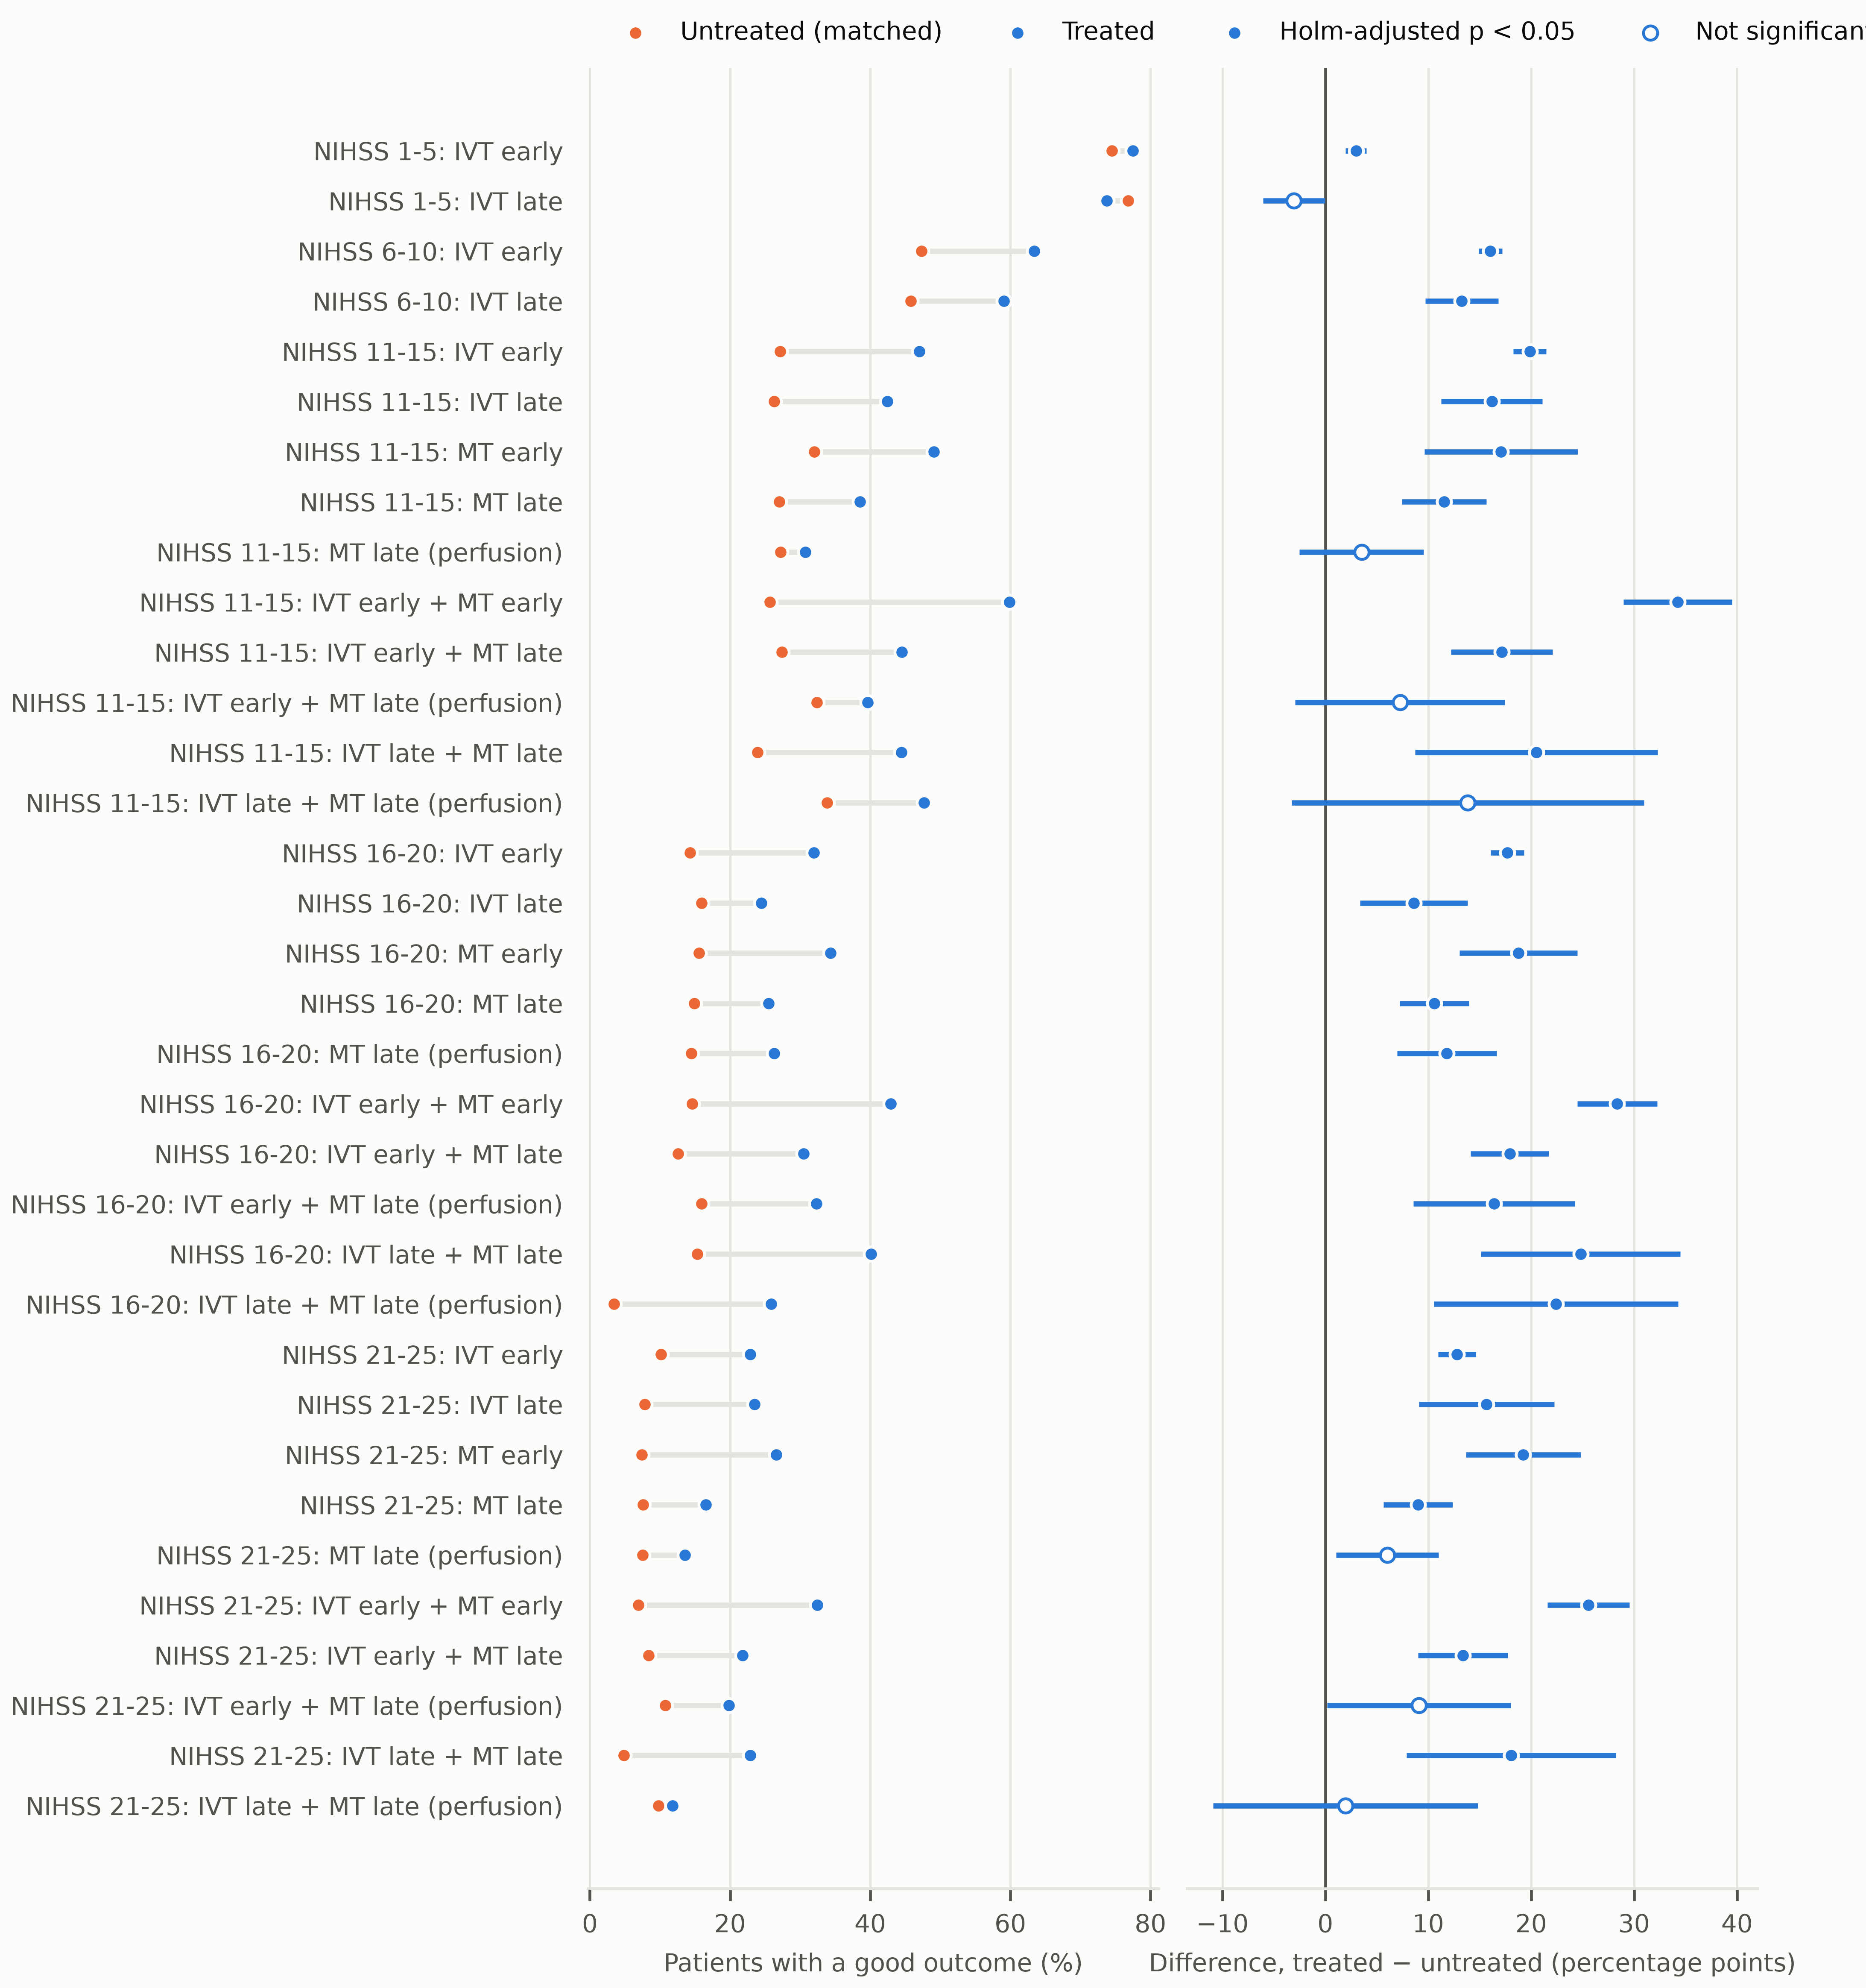
\includegraphics[width=1\linewidth]{chapters/images/all_ischaemic_stroke_target_trials_outcome_target_chart.png}
\caption{Good outcome at discharge (mRS $\le$ 2, or no worse than before the stroke) in each trial group. Left: percentage of treated patients (blue) and matched untreated controls (orange) with a good outcome. Right: difference between arms (treated minus untreated, percentage points) with 95\% confidence interval; filled markers show a Holm-adjusted $p < 0.05$ (McNemar's test). Higher is better. Full results are given in Supplementary Table~\ref{tab:supp_outcome_target}.}
\label{fig:outcome_target}
{\small\textit{Alt text:} Two-panel dot plot for 34 trial groups ordered by stroke severity band. The left panel shows the percentage of treated and matched untreated patients with a good outcome at discharge. The right panel shows the difference in percentage points with 95\% confidence intervals. Most differences are positive, and the largest are for early thrombolysis plus early thrombectomy in moderate to severe stroke.\par}
\end{figure}

% Death

\begin{figure}
\centering
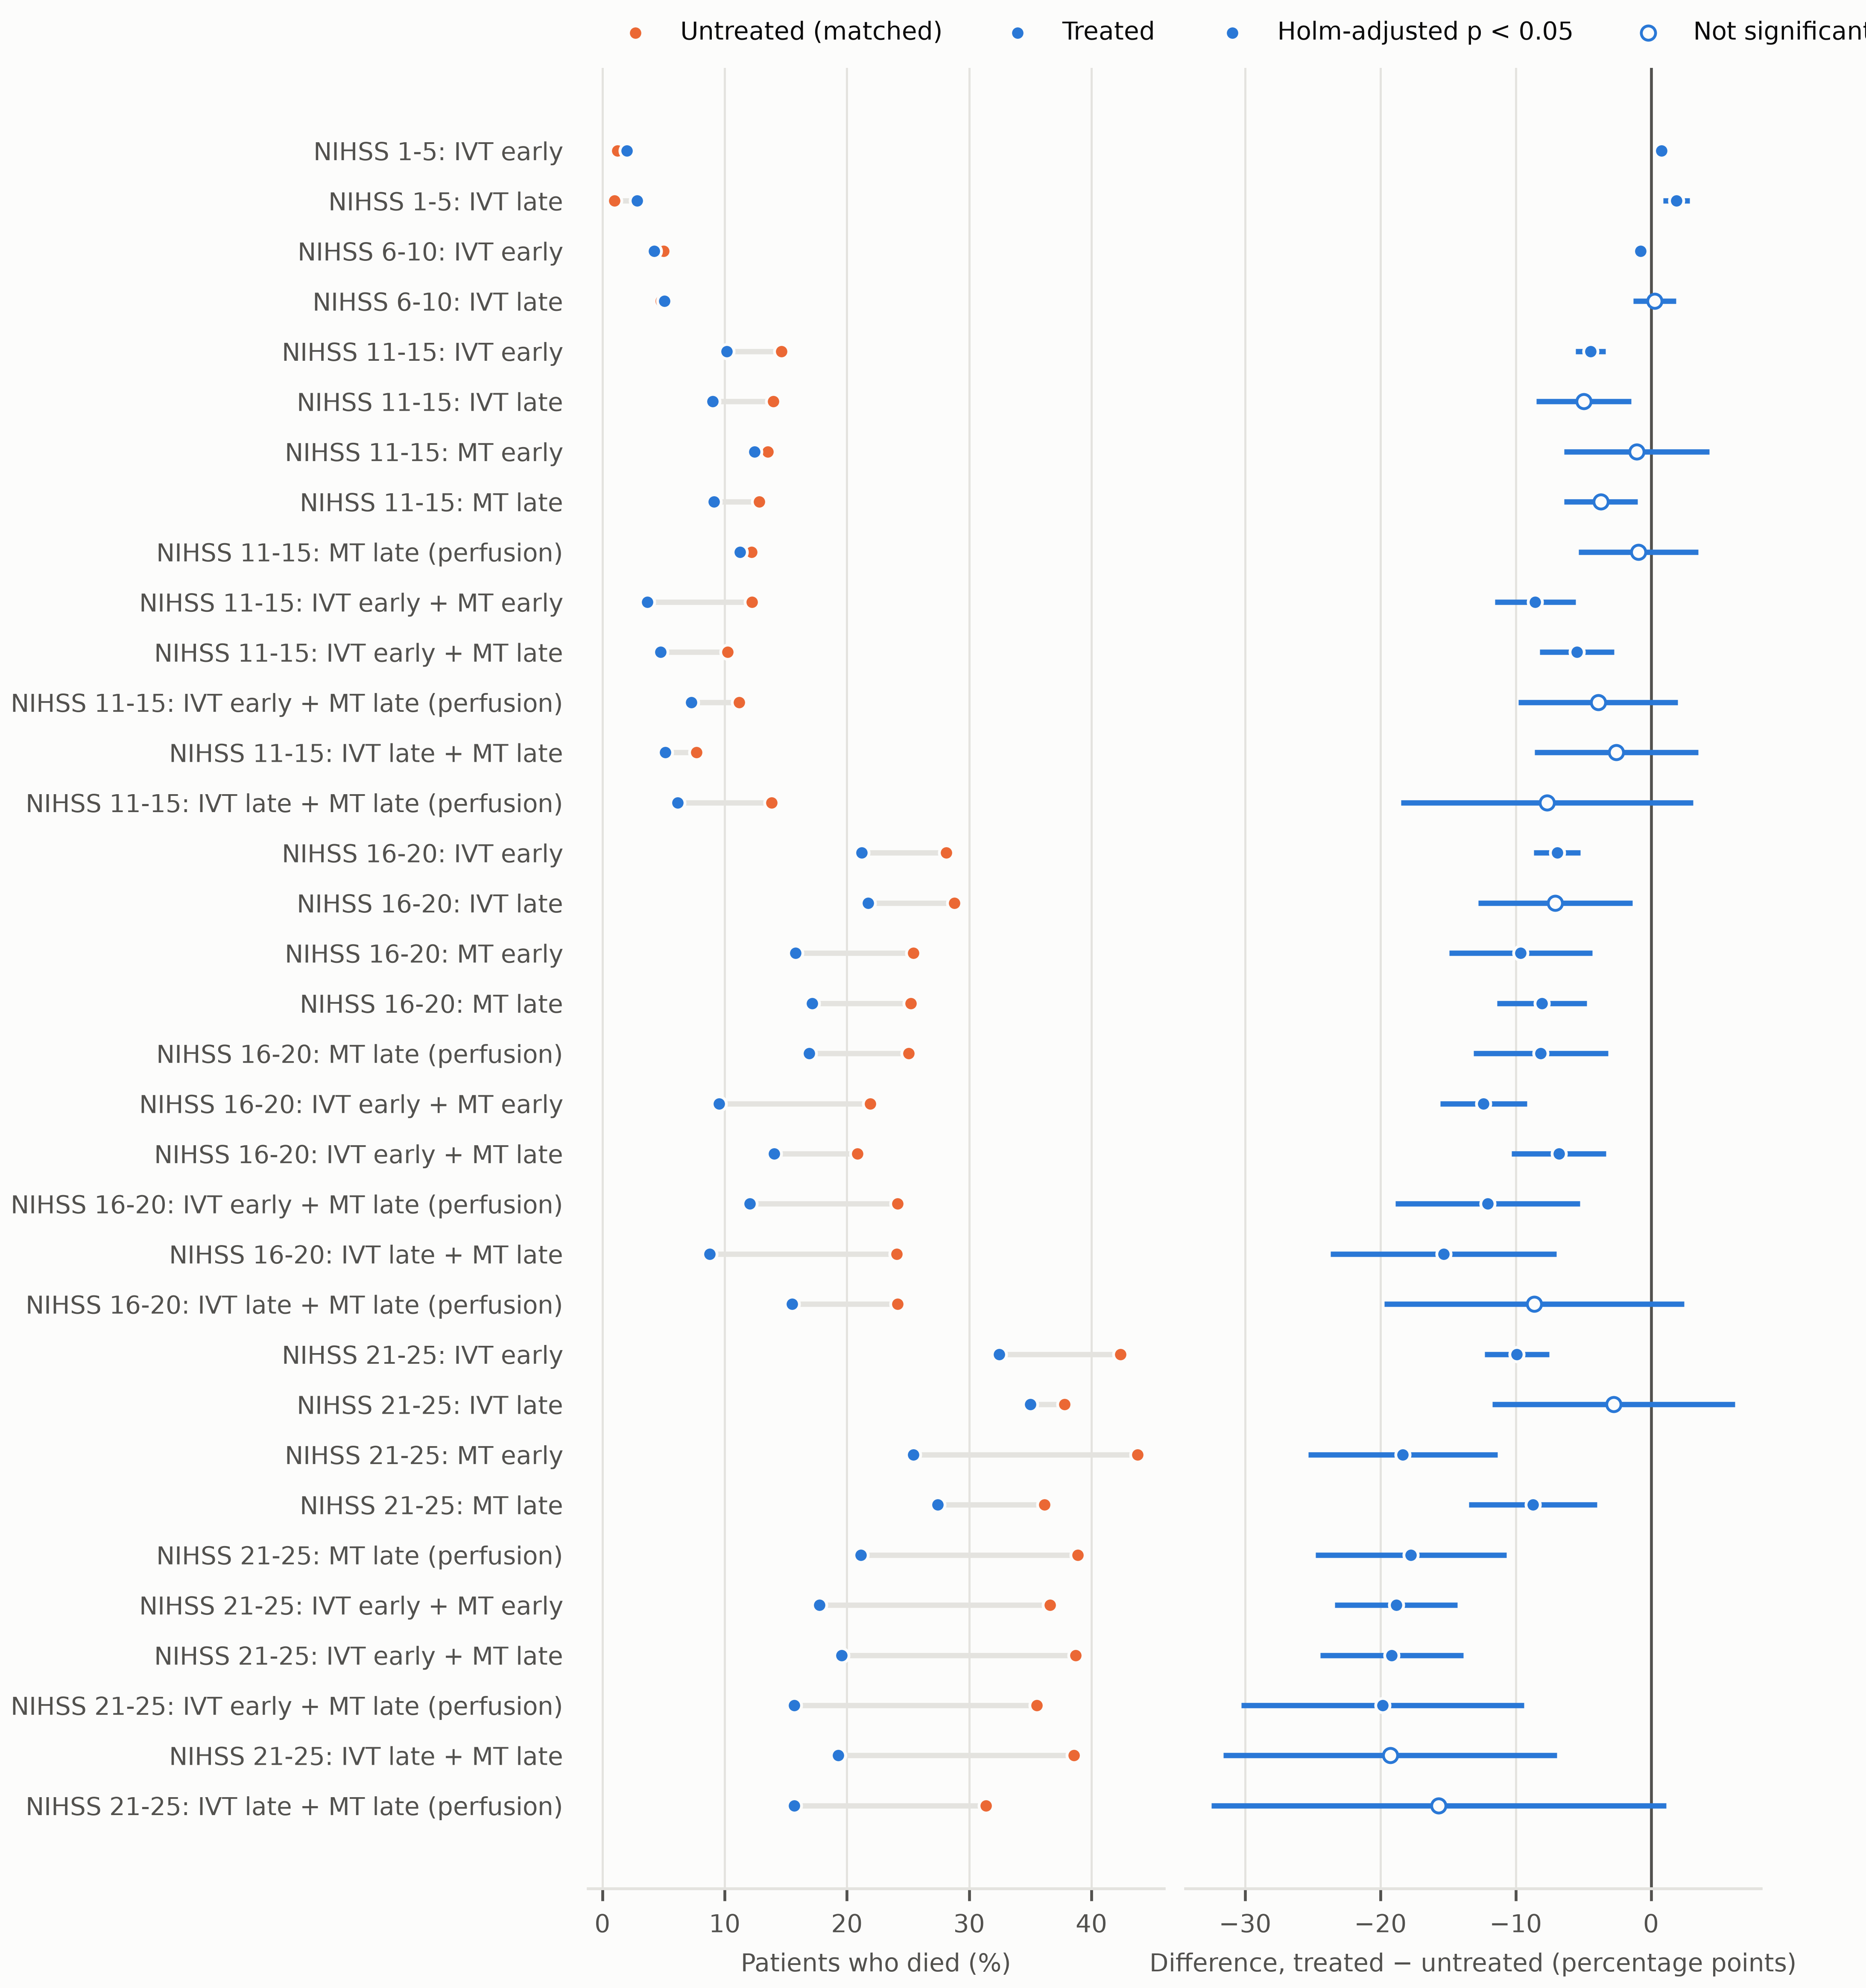
\includegraphics[width=1\linewidth]{chapters/images/all_ischaemic_stroke_target_trials_death_chart.png}
\caption{In-hospital death in each trial group. Left: percentage of treated patients (blue) and matched untreated controls (orange) who died in hospital. Right: difference between arms (treated minus untreated, percentage points) with 95\% confidence interval; filled markers show a Holm-adjusted $p < 0.05$ (McNemar's test). Lower is better. Full results are given in Supplementary Table~\ref{tab:supp_death}.}
\label{fig:death}
{\small\textit{Alt text:} Two-panel dot plot for 34 trial groups ordered by stroke severity band. The left panel shows the percentage of treated and matched untreated patients who died in hospital. The right panel shows the difference in percentage points with 95\% confidence intervals. Deaths are slightly more common with thrombolysis in mild stroke and less common with treatment in most moderate and severe stroke groups.\par}
\end{figure}

% Discharge disability

\begin{figure}
\centering
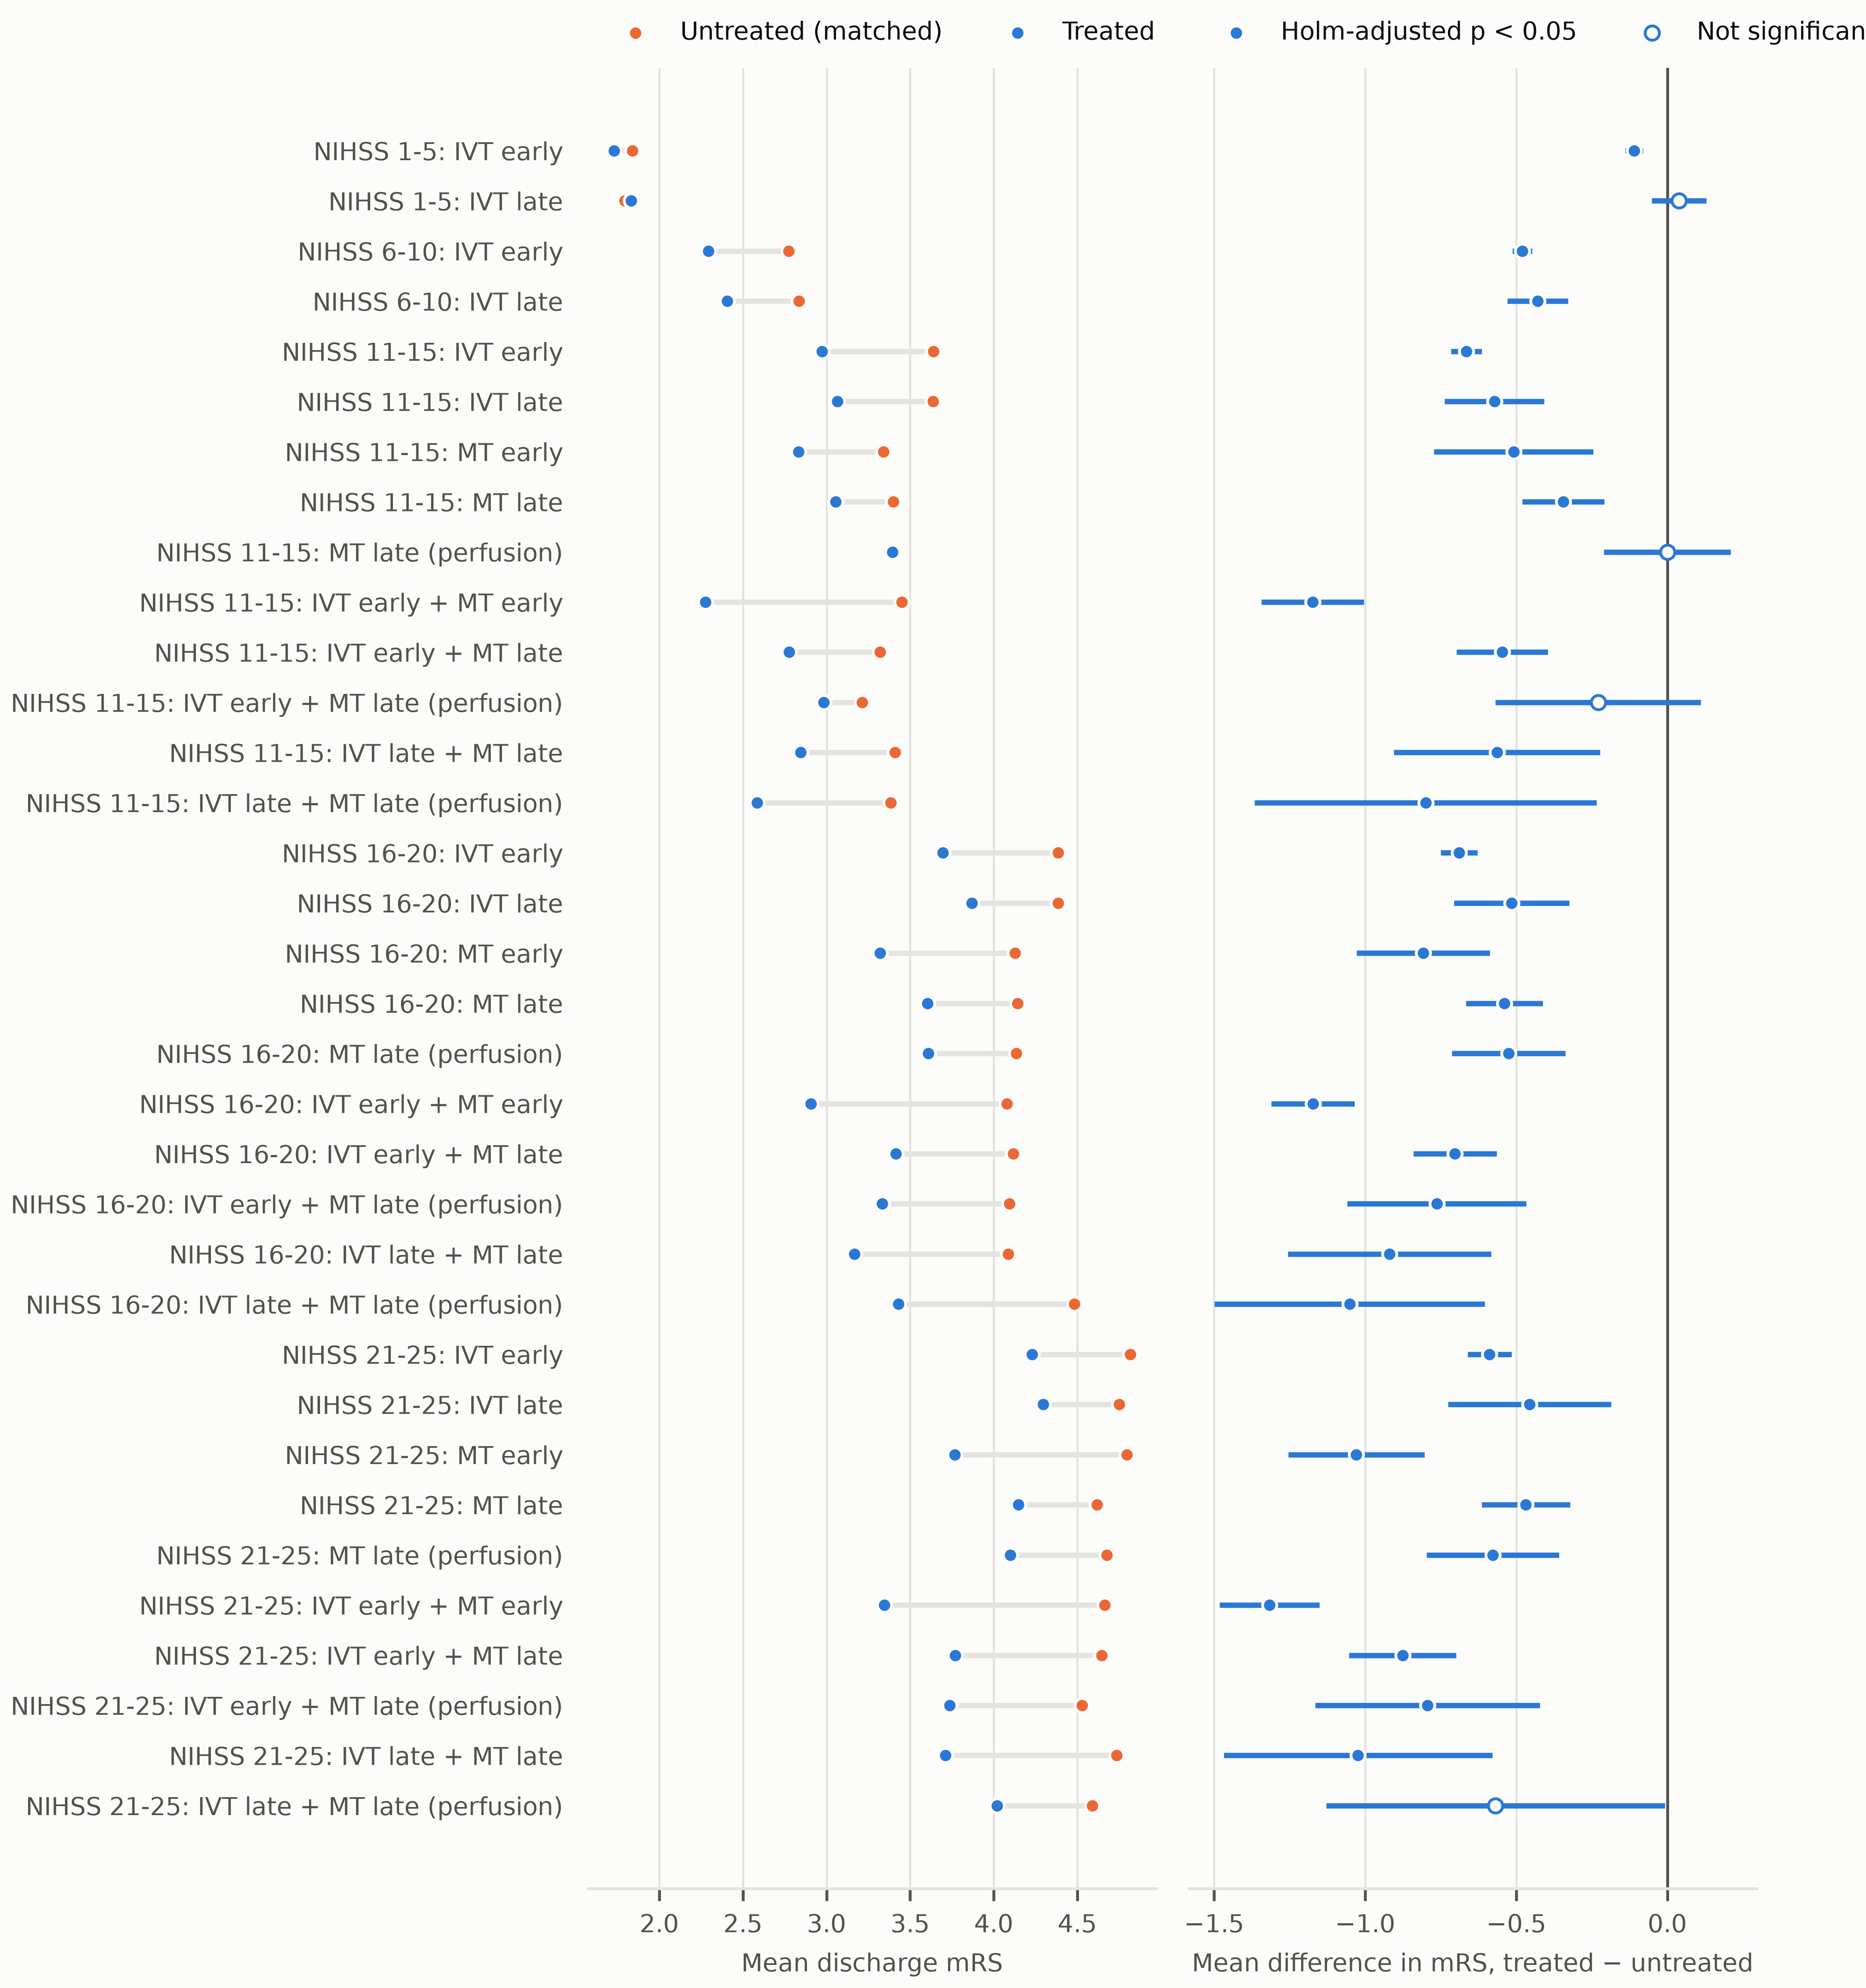
\includegraphics[width=1\linewidth]{chapters/images/all_ischaemic_stroke_target_trials_discharge_disability_chart.png}
\caption{Disability at discharge (modified Rankin Scale, 0--6) in each trial group. Left: mean discharge mRS of treated patients (blue) and matched untreated controls (orange). Right: mean within-pair difference (treated minus untreated) with 95\% confidence interval; filled markers show a Holm-adjusted $p < 0.05$ (Wilcoxon signed-rank test). Lower is better. Full results are given in Supplementary Table~\ref{tab:supp_discharge_disability}.}
\label{fig:discharge_disability}
{\small\textit{Alt text:} Two-panel dot plot for 34 trial groups ordered by stroke severity band. The left panel shows mean modified Rankin Scale score at discharge in treated and matched untreated patients. The right panel shows the mean difference with 95\% confidence intervals. Treated patients have lower scores in most groups, with the largest reductions for early thrombolysis plus early thrombectomy.\par}
\end{figure}

% Length of stay

\begin{figure}
\centering
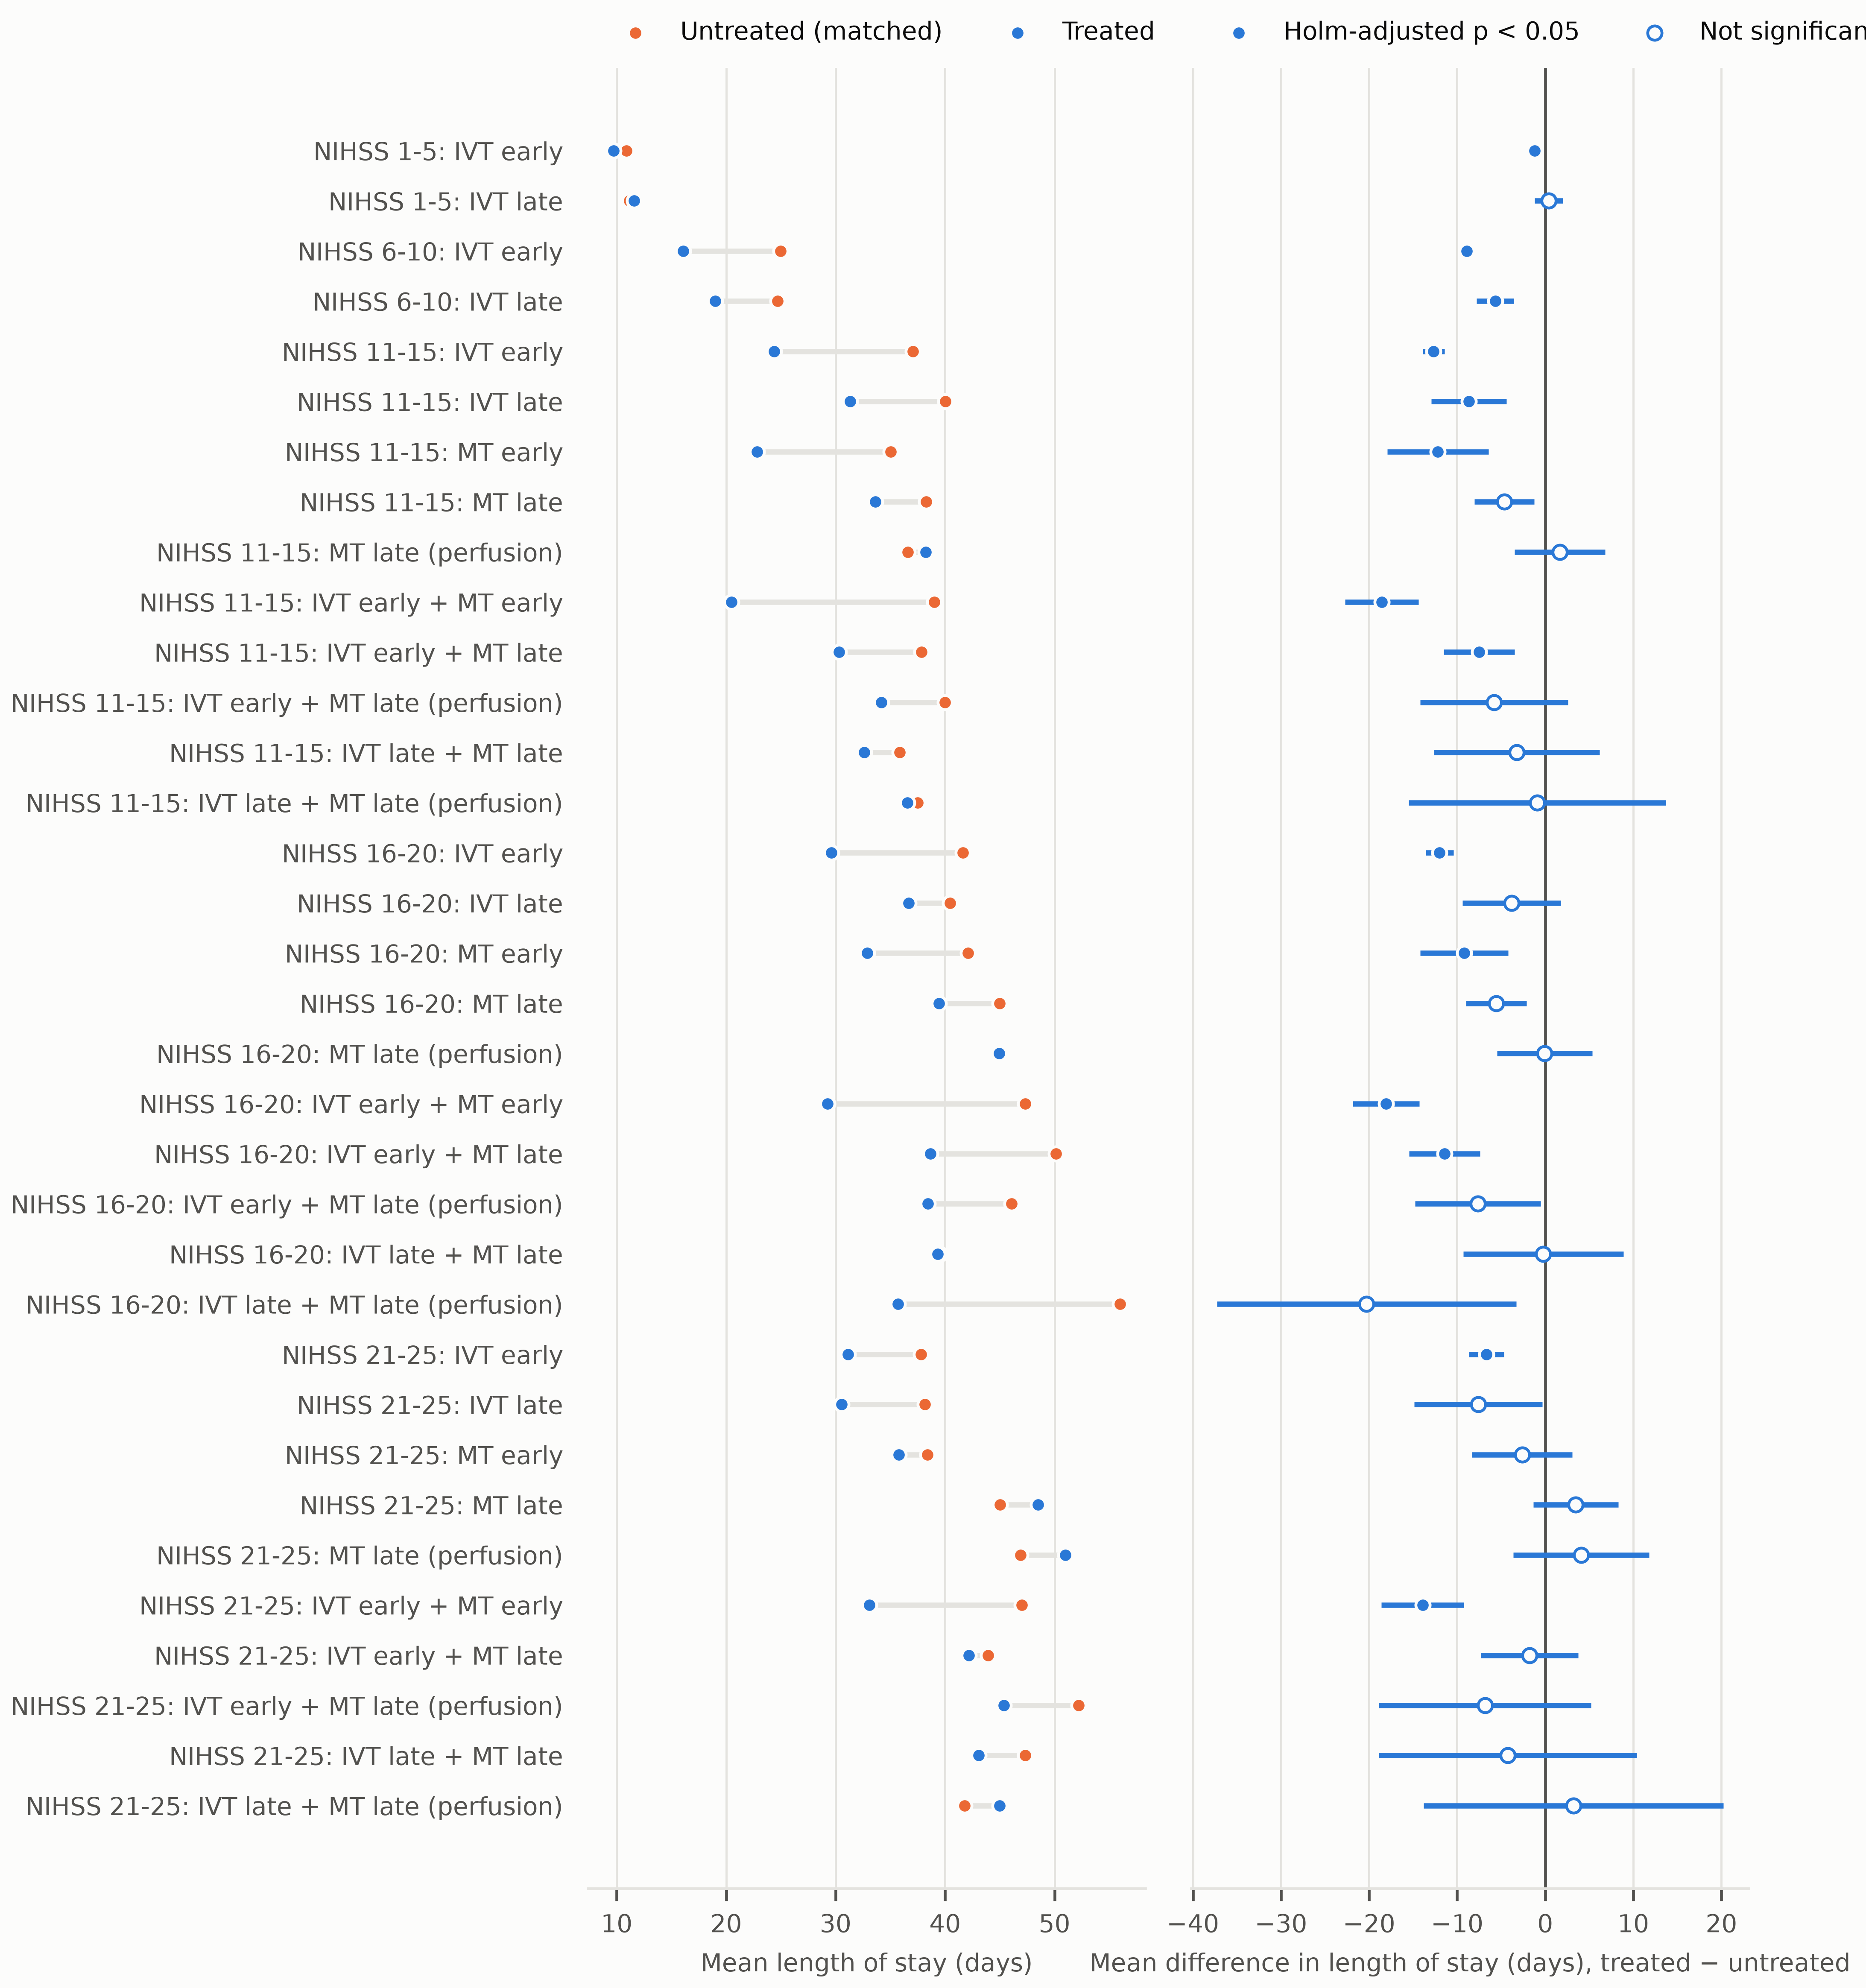
\includegraphics[width=1\linewidth]{chapters/images/all_ischaemic_stroke_target_trials_length_of_stay_chart.png}
\caption{Length of hospital stay (days) in each trial group, including patients who died in hospital. Left: mean length of stay of treated patients (blue) and matched untreated controls (orange). Right: mean within-pair difference (treated minus untreated, days) with 95\% confidence interval; filled markers show a Holm-adjusted $p < 0.05$ (Wilcoxon signed-rank test). Full results are given in Supplementary Table~\ref{tab:supp_length_of_stay}.}
\label{fig:length_of_stay}
{\small\textit{Alt text:} Two-panel dot plot for 34 trial groups ordered by stroke severity band. The left panel shows mean length of hospital stay in days for treated and matched untreated patients. The right panel shows the mean difference in days with 95\% confidence intervals. Stays are shorter with treatment in most groups, by up to about 18 days.\par}
\end{figure}

% Discharge destination

\begin{figure}
\centering
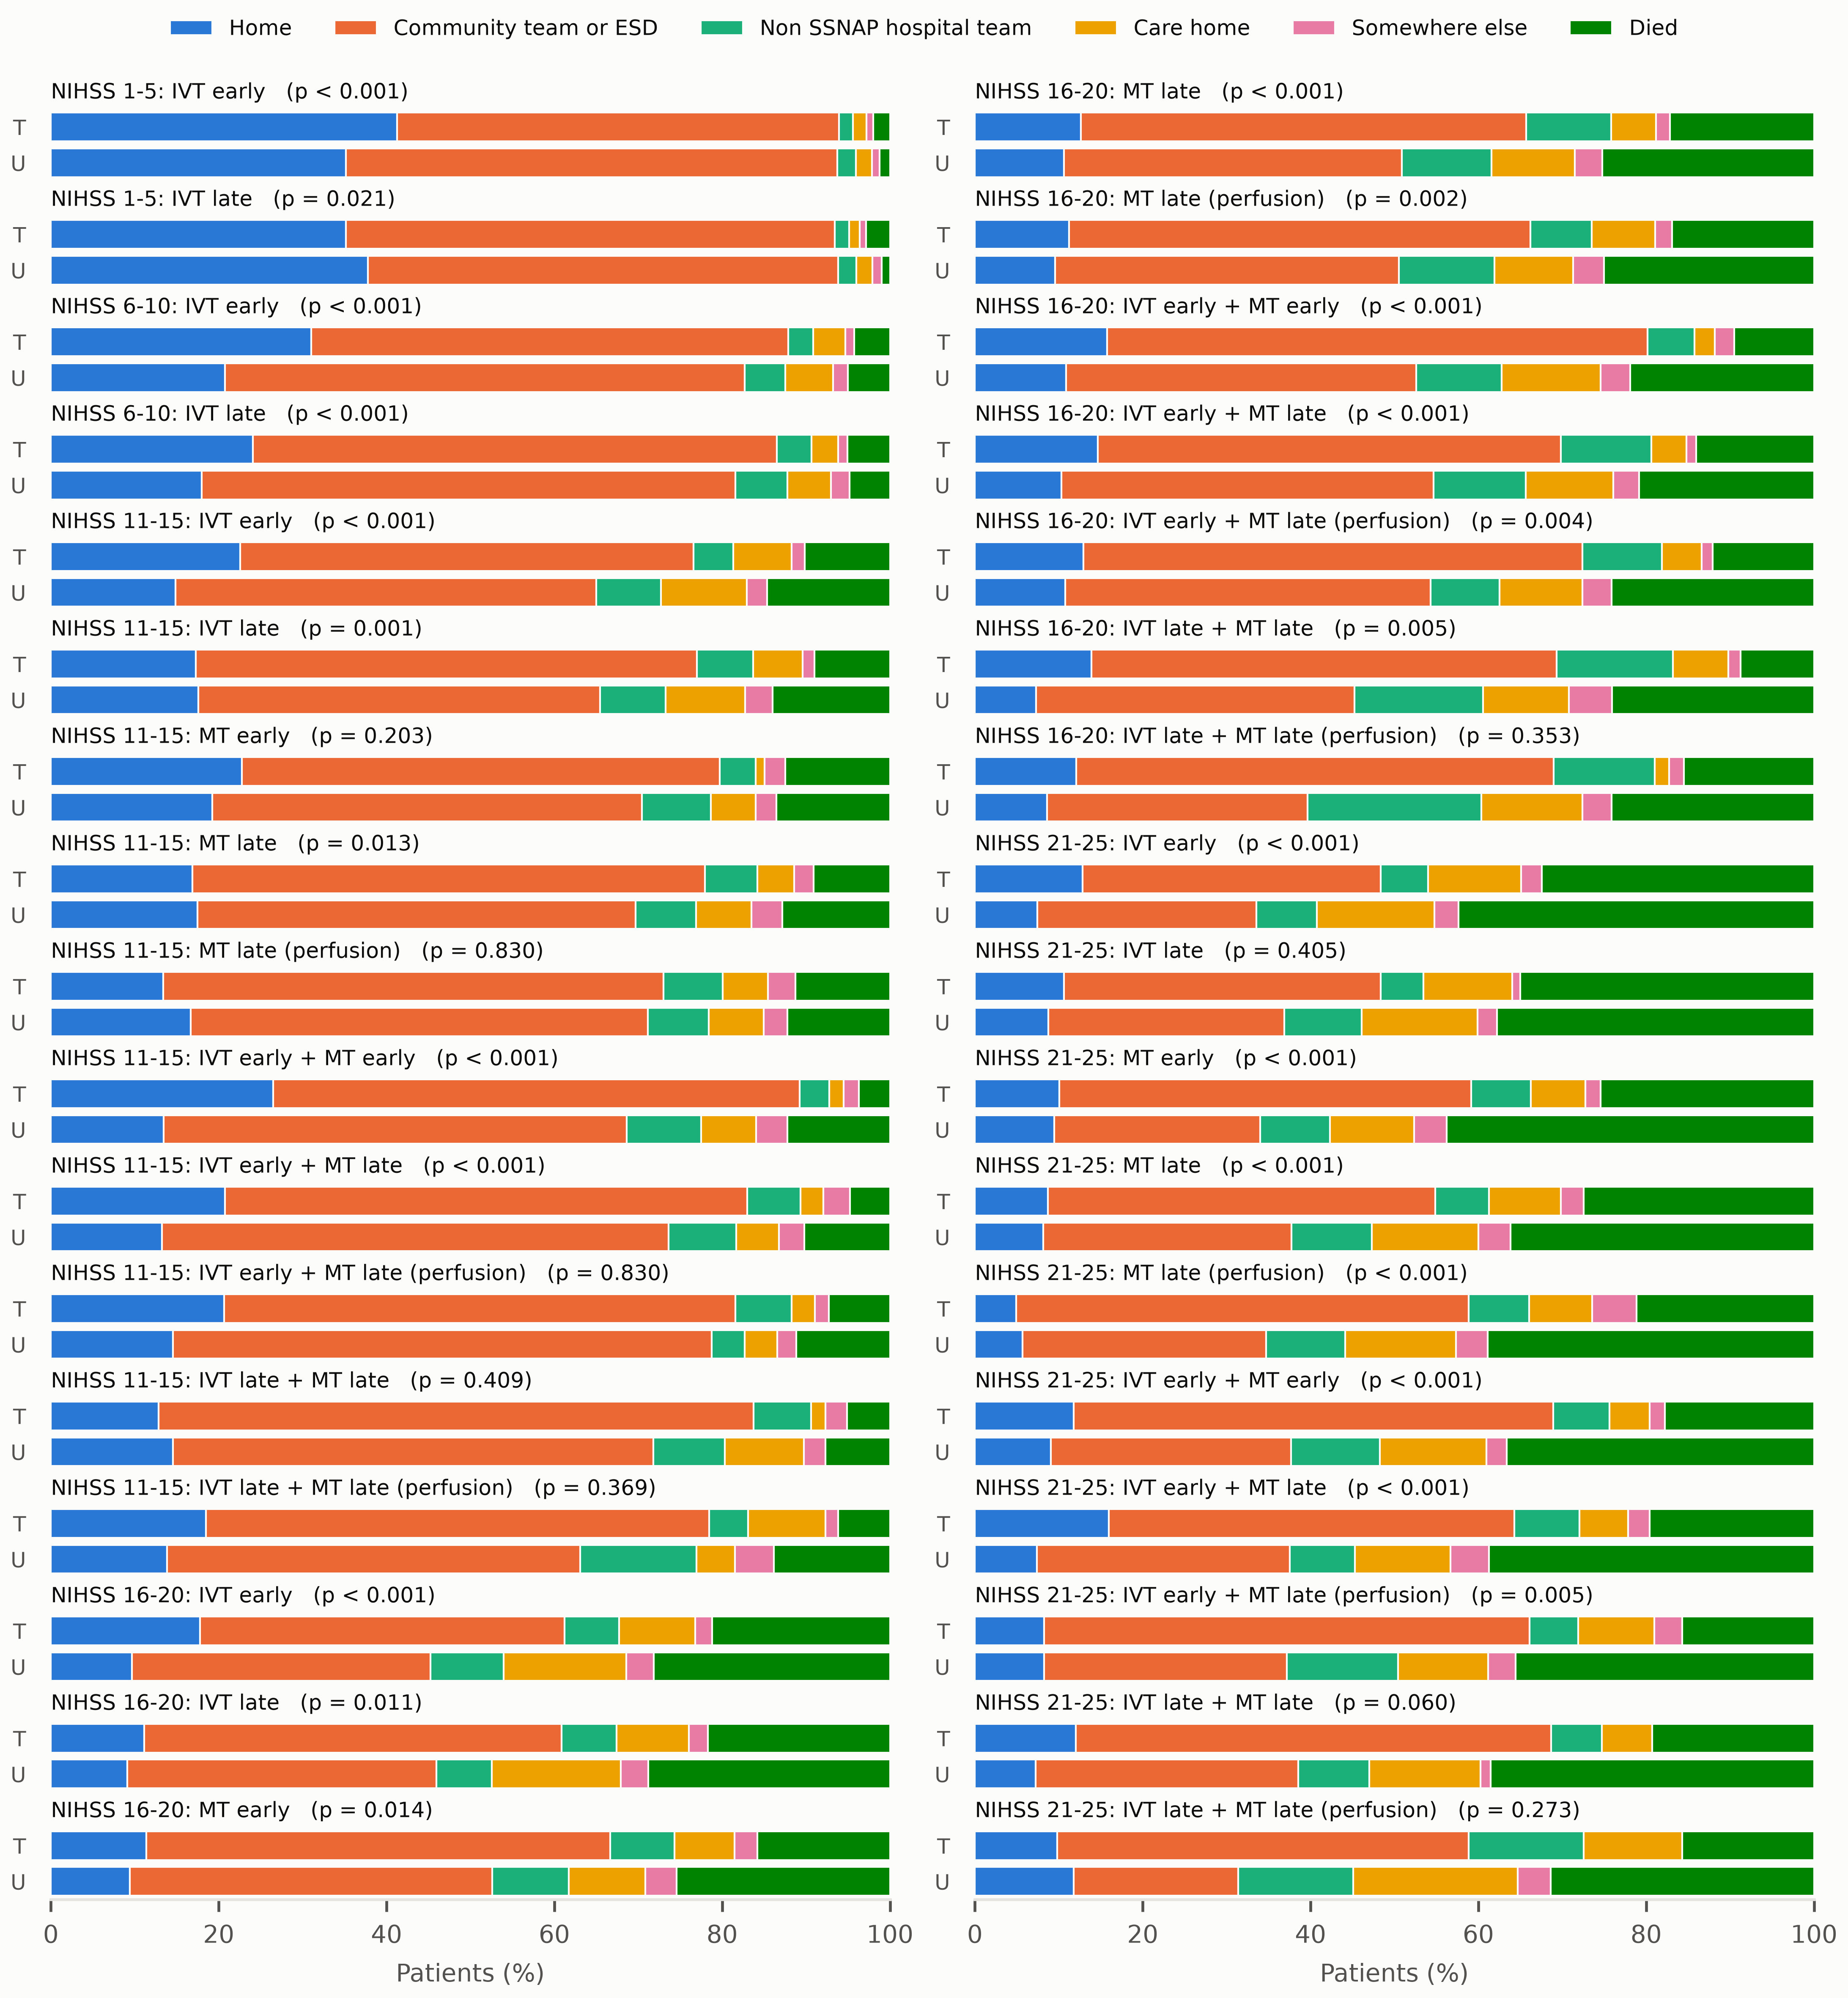
\includegraphics[width=1\linewidth,height=0.75\textheight,keepaspectratio]{chapters/images/all_ischaemic_stroke_target_trials_discharge_destination_chart.png}
\caption{Discharge destination in each trial group. Bars show the percentage of patients discharged to each destination for the treated (T) and matched untreated (U) arm of each group. The Holm-adjusted $p$-value from the Stuart--Maxwell test of marginal homogeneity is given after each group name. ESD, early supported discharge. Full results are given in Supplementary Table~\ref{tab:supp_discharge_destination}.}
\label{fig:discharge_destination}
{\small\textit{Alt text:} Horizontal stacked bar chart in two panels, with a pair of bars, treated and matched untreated, for each of 34 trial groups. Each bar shows the percentage discharged home, with community team or early supported discharge, to another hospital team, to a care home, elsewhere, or who died. Treated patients more often went home and less often went to a care home or died.\par}
\end{figure}
